

\tikzset{every picture/.style={line width=0.75pt}} %set default line width to 0.75pt        

\begin{figure}[H]
\caption{Grafo di De Brujin}
\begin{center}
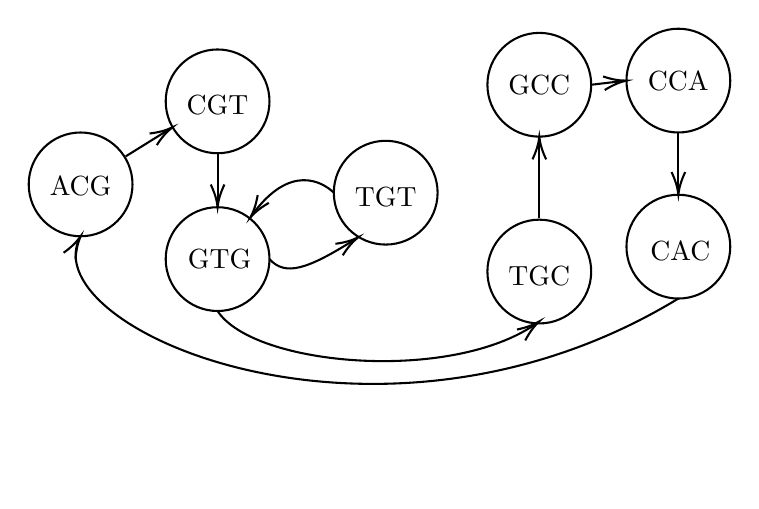
\begin{tikzpicture}[x=0.75pt,y=0.75pt,yscale=-1,xscale=1]
%uncomment if require: \path (0,248); %set diagram left start at 0, and has height of 248

%Shape: Circle [id:dp5662414203096264] 
\draw   (81,53) .. controls (81,39.19) and (92.19,28) .. (106,28) .. controls (119.81,28) and (131,39.19) .. (131,53) .. controls (131,66.81) and (119.81,78) .. (106,78) .. controls (92.19,78) and (81,66.81) .. (81,53) -- cycle ;
%Shape: Circle [id:dp13985089677551477] 
\draw   (81,129) .. controls (81,115.19) and (92.19,104) .. (106,104) .. controls (119.81,104) and (131,115.19) .. (131,129) .. controls (131,142.81) and (119.81,154) .. (106,154) .. controls (92.19,154) and (81,142.81) .. (81,129) -- cycle ;
%Shape: Circle [id:dp3574816316500795] 
\draw   (15,93) .. controls (15,79.19) and (26.19,68) .. (40,68) .. controls (53.81,68) and (65,79.19) .. (65,93) .. controls (65,106.81) and (53.81,118) .. (40,118) .. controls (26.19,118) and (15,106.81) .. (15,93) -- cycle ;
%Shape: Circle [id:dp6367614117013465] 
\draw   (162,97) .. controls (162,83.19) and (173.19,72) .. (187,72) .. controls (200.81,72) and (212,83.19) .. (212,97) .. controls (212,110.81) and (200.81,122) .. (187,122) .. controls (173.19,122) and (162,110.81) .. (162,97) -- cycle ;
%Shape: Circle [id:dp8286860889666687] 
\draw   (236,135) .. controls (236,121.19) and (247.19,110) .. (261,110) .. controls (274.81,110) and (286,121.19) .. (286,135) .. controls (286,148.81) and (274.81,160) .. (261,160) .. controls (247.19,160) and (236,148.81) .. (236,135) -- cycle ;
%Shape: Circle [id:dp04605576669499256] 
\draw   (236,45) .. controls (236,31.19) and (247.19,20) .. (261,20) .. controls (274.81,20) and (286,31.19) .. (286,45) .. controls (286,58.81) and (274.81,70) .. (261,70) .. controls (247.19,70) and (236,58.81) .. (236,45) -- cycle ;
%Shape: Circle [id:dp9155218336299027] 
\draw   (303,43) .. controls (303,29.19) and (314.19,18) .. (328,18) .. controls (341.81,18) and (353,29.19) .. (353,43) .. controls (353,56.81) and (341.81,68) .. (328,68) .. controls (314.19,68) and (303,56.81) .. (303,43) -- cycle ;
%Shape: Circle [id:dp766738912437283] 
\draw   (303,123) .. controls (303,109.19) and (314.19,98) .. (328,98) .. controls (341.81,98) and (353,109.19) .. (353,123) .. controls (353,136.81) and (341.81,148) .. (328,148) .. controls (314.19,148) and (303,136.81) .. (303,123) -- cycle ;
%Straight Lines [id:da9646625679785032] 
\draw    (61.75,79.5) -- (82.55,66.56) ;
\draw [shift={(84.25,65.5)}, rotate = 508.11] [color={rgb, 255:red, 0; green, 0; blue, 0 }  ][line width=0.75]    (10.93,-3.29) .. controls (6.95,-1.4) and (3.31,-0.3) .. (0,0) .. controls (3.31,0.3) and (6.95,1.4) .. (10.93,3.29)   ;

%Straight Lines [id:da8830983152823235] 
\draw    (106,78) -- (106,102) ;
\draw [shift={(106,104)}, rotate = 270] [color={rgb, 255:red, 0; green, 0; blue, 0 }  ][line width=0.75]    (10.93,-3.29) .. controls (6.95,-1.4) and (3.31,-0.3) .. (0,0) .. controls (3.31,0.3) and (6.95,1.4) .. (10.93,3.29)   ;

%Curve Lines [id:da7743744950450349] 
\draw    (131,129) .. controls (138.6,137.33) and (149.07,134.14) .. (172.31,119.42) ;
\draw [shift={(173.75,118.5)}, rotate = 507.41] [color={rgb, 255:red, 0; green, 0; blue, 0 }  ][line width=0.75]    (10.93,-3.29) .. controls (6.95,-1.4) and (3.31,-0.3) .. (0,0) .. controls (3.31,0.3) and (6.95,1.4) .. (10.93,3.29)   ;

%Curve Lines [id:da701157029011428] 
\draw    (162,97) .. controls (156.37,91.61) and (140.89,82.86) .. (122.86,107.45) ;
\draw [shift={(121.75,109)}, rotate = 304.92] [color={rgb, 255:red, 0; green, 0; blue, 0 }  ][line width=0.75]    (10.93,-3.29) .. controls (6.95,-1.4) and (3.31,-0.3) .. (0,0) .. controls (3.31,0.3) and (6.95,1.4) .. (10.93,3.29)   ;

%Curve Lines [id:da9534415928320956] 
\draw    (328,148) .. controls (184.94,235.12) and (18.86,163.46) .. (39.32,119.33) ;
\draw [shift={(40,118)}, rotate = 479.11] [color={rgb, 255:red, 0; green, 0; blue, 0 }  ][line width=0.75]    (10.93,-3.29) .. controls (6.95,-1.4) and (3.31,-0.3) .. (0,0) .. controls (3.31,0.3) and (6.95,1.4) .. (10.93,3.29)   ;

%Curve Lines [id:da9799576589537213] 
\draw    (106,154) .. controls (123.33,180.73) and (219.06,188.84) .. (259.78,159.89) ;
\draw [shift={(261,159)}, rotate = 503.13] [color={rgb, 255:red, 0; green, 0; blue, 0 }  ][line width=0.75]    (10.93,-3.29) .. controls (6.95,-1.4) and (3.31,-0.3) .. (0,0) .. controls (3.31,0.3) and (6.95,1.4) .. (10.93,3.29)   ;

%Straight Lines [id:da2213126680718589] 
\draw    (261,109) -- (261,72) ;
\draw [shift={(261,70)}, rotate = 450] [color={rgb, 255:red, 0; green, 0; blue, 0 }  ][line width=0.75]    (10.93,-3.29) .. controls (6.95,-1.4) and (3.31,-0.3) .. (0,0) .. controls (3.31,0.3) and (6.95,1.4) .. (10.93,3.29)   ;

%Straight Lines [id:da05405134063421202] 
\draw    (328,96) -- (328,68) ;

\draw [shift={(328,98)}, rotate = 270] [color={rgb, 255:red, 0; green, 0; blue, 0 }  ][line width=0.75]    (10.93,-3.29) .. controls (6.95,-1.4) and (3.31,-0.3) .. (0,0) .. controls (3.31,0.3) and (6.95,1.4) .. (10.93,3.29)   ;
%Straight Lines [id:da7142573004014958] 
\draw    (286,45) -- (301.01,43.23) ;
\draw [shift={(303,43)}, rotate = 533.29] [color={rgb, 255:red, 0; green, 0; blue, 0 }  ][line width=0.75]    (10.93,-3.29) .. controls (6.95,-1.4) and (3.31,-0.3) .. (0,0) .. controls (3.31,0.3) and (6.95,1.4) .. (10.93,3.29)   ;


% Text Node
\draw (40,94) node  [align=left] {ACG};
% Text Node
\draw (106,55) node  [align=left] {CGT};
% Text Node
\draw (107,129) node  [align=left] {GTG};
% Text Node
\draw (187,99) node  [align=left] {TGT};
% Text Node
\draw (261,45) node  [align=left] {GCC};
% Text Node
\draw (328,43) node  [align=left] {CCA};
% Text Node
\draw (261,137) node  [align=left] {TGC};
% Text Node
\draw (329,125) node  [align=left] {CAC};


\end{tikzpicture}
\end{center}
\end{figure}